\documentclass[tikz, border=3.14mm]{standalone}
\usepackage{pgfplots}
\pgfplotsset{compat=1.18}

\begin{document}
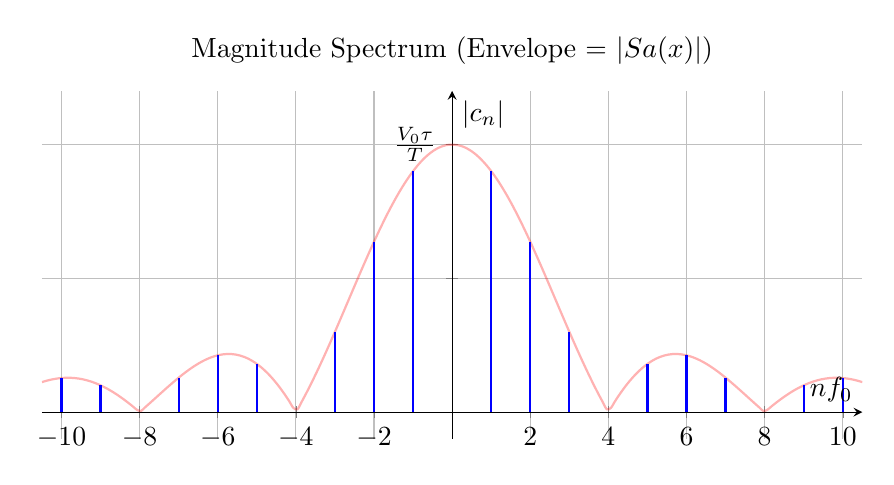
\begin{tikzpicture}
    \begin{axis}[
        axis lines = middle,
        xlabel = {$n f_0$},
        ylabel = {$|c_n|$},
        xmin = -10.5, xmax = 10.5,
        ymin = -0.1, ymax = 1.2,
        xtick = {-10, -8, -6, -4, -2, 0, 2, 4, 6, 8, 10},
        ytick = {0, 0.5, 1},
        yticklabels = {0, , $\frac{V_0 \tau}{T}$},
        grid = major,
        width = 12cm,
        height = 6cm,
        title = {Magnitude Spectrum (Envelope = $|Sa(x)|$)}
    ]
        % Envelope: Sa(x) = sin(x)/x where x = pi * f * tau
        % Let's assume tau = 0.25 (crosses at f = 4, 8, ...)
        \addplot[thick, red, smooth, domain=-10.5:10.5, samples=200, opacity=0.3] {abs(sin(3.1415*x*0.25*180/3.1415)/(3.1415*x*0.25))};
        
        % Discrete lines at n*f0 (assume f0 = 1)
        \foreach \n in {-10,-9,...,10} {
            \addplot[blue, thick, ycomb, samples at={\n}] {abs(sin(3.1415*x*0.25*180/3.1415)/(3.1415*x*0.25))};
        }
    \end{axis}
\end{tikzpicture}
\end{document}
